\PassOptionsToPackage{table}{xcolor}
\documentclass{rapportFSR}
\usepackage[utf8]{inputenc}
\usepackage[T1]{fontenc}
\usepackage{lipsum}
\usepackage{mdframed}
\usepackage{tcolorbox}
\usepackage{pifont}
\usepackage{fontawesome5}
\usepackage{listings}
\usepackage{xcolor}
\usepackage{colortbl}
\usepackage{tikz}
\usetikzlibrary{shapes.geometric,arrows.meta,positioning,fit,backgrounds,calc}

% Palette de couleurs harmonieuse
\definecolor{header}{RGB}{40,60,120}
\definecolor{rowgray}{RGB}{245,245,245}
\definecolor{lightblue}{RGB}{225,235,255}
\definecolor{lightgreen}{RGB}{230,245,230}
\definecolor{lightorange}{RGB}{255,243,230}
\definecolor{darkblue}{RGB}{20,40,90}
\definecolor{codebg}{RGB}{248,249,250}
\definecolor{framecolor}{RGB}{220,224,230}
\definecolor{javapurple}{RGB}{127,0,85}
\definecolor{javagreen}{RGB}{63,127,95}
\definecolor{javared}{RGB}{190,40,40}
\definecolor{javablue}{RGB}{0,80,160}

% Configuration des styles de code
\lstdefinestyle{console}{
    backgroundcolor=\color{black!5},
    basicstyle=\ttfamily\footnotesize,
    frame=single,
    rulecolor=\color{black!20},
    breaklines=true,
    columns=fullflexible
}

\lstdefinestyle{java}{
    backgroundcolor=\color{codebg},
    basicstyle=\ttfamily\scriptsize,
    keywordstyle=\color{javapurple}\bfseries,
    stringstyle=\color{javared},
    commentstyle=\color{javagreen}\itshape,
    morecomment=[s][\color{javablue}]{/**}{*/},
    numbers=left,
    numberstyle=\tiny\color{gray},
    numbersep=6pt,
    frame=single,
    rulecolor=\color{framecolor},
    breaklines=true,
    breakatwhitespace=true,
    showstringspaces=false,
    tabsize=4
}

\lstdefinestyle{properties}{
    backgroundcolor=\color{codebg},
    basicstyle=\ttfamily\scriptsize,
    keywordstyle=\color{darkblue}\bfseries,
    commentstyle=\color{javagreen}\itshape,
    numbers=left,
    numberstyle=\tiny\color{gray},
    numbersep=6pt,
    frame=single,
    rulecolor=\color{framecolor},
    breaklines=true,
    showstringspaces=false
}

\title{Rapport - TP Spring Security \& JWT}

\begin{document}

%------------------ Informations du TP ------------------
\titre{Sécurisation d'une API REST avec Spring Security 6 \& JWT} 
\sujet{} 
\enseignant{Pr. Abdelmajid \textsc{BOUSSELHAM}} 
\eleves{Ayoub \textsc{ELHOUANI}} 

\fairemarges
\fairepagedegarde
\tabledematieres
\newpage
\listoffigures
\newpage

%------------------ Section 1 : Introduction & Architecture ------------------
\section{Architecture Globale \& Authentification Stateless}

\subsection{Objectif \& Problématique}
L'approche \textbf{JWT (RFC 7519)} permet de déporter la preuve d'identité chez le client dans un modèle sans état (\textit{Stateless}). Contrairement à l'authentification avec état (\textit{Stateful}) basée sur les sessions HTTP en mémoire serveur (\texttt{JSESSIONID}) qui entrave le passage à l'échelle horizontal (\textit{horizontal scalability}), chaque requête est auto-suffisante et validée cryptographiquement à la volée par les filtres de sécurité.

\subsection{Schéma d'Architecture Globale en Couches}
La figure~\ref{fig:arch-globale} synthétise l'architecture en couches mise en place dans notre projet.

\begin{figure}[H]
\centering
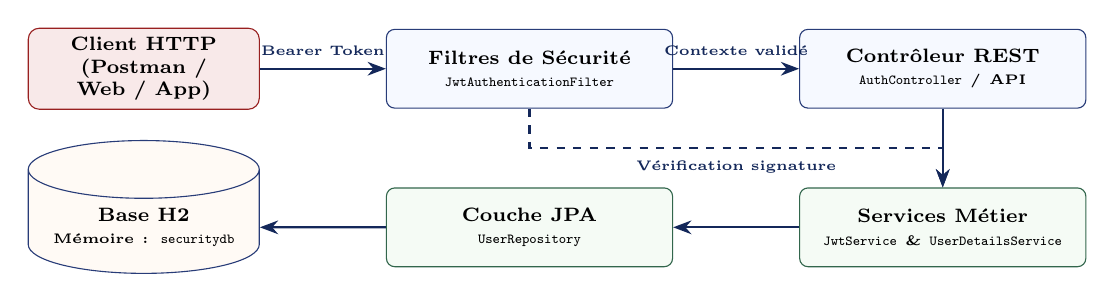
\begin{tikzpicture}[
    node distance=1cm and 1.6cm,
    block/.style={rectangle, draw=header, fill=lightblue!30, text width=3.4cm, text centered, rounded corners=3pt, minimum height=1cm, font=\scriptsize\bfseries},
    service/.style={rectangle, draw=javagreen!80!black, fill=lightgreen!40, text width=3.4cm, text centered, rounded corners=3pt, minimum height=1cm, font=\scriptsize\bfseries},
    db/.style={cylinder, draw=header, fill=lightorange!40, shape border rotate=90, aspect=0.25, text width=2.7cm, text centered, minimum height=1.1cm, font=\scriptsize\bfseries},
    client/.style={rectangle, draw=javared!80!black, fill=javared!10, text width=2.7cm, text centered, rounded corners=4pt, minimum height=1cm, font=\scriptsize\bfseries},
    arrow/.style={-Stealth, thick, color=darkblue}
]

\node[client] (client) {Client HTTP\\(Postman / Web / App)};
\node[block, right=of client] (filter) {Filtres de Sécurité\\{\tiny \texttt{JwtAuthenticationFilter}}};
\node[block, right=of filter] (ctrl) {Contrôleur REST\\{\tiny \texttt{AuthController} / API}};
\node[service, below=1cm of ctrl] (service) {Services Métier\\{\tiny \texttt{JwtService} \& \texttt{UserDetailsService}}};
\node[service, left=of service] (repo) {Couche JPA\\{\tiny \texttt{UserRepository}}};
\node[db, left=of repo] (db) {Base H2\\{\tiny Mémoire : \texttt{securitydb}}};

\draw[arrow] (client) -- node[above=1pt, font=\tiny\bfseries] {Bearer Token} (filter);
\draw[arrow] (filter) -- node[above=1pt, font=\tiny\bfseries] {Contexte validé} (ctrl);
\draw[arrow] (ctrl) -- (service);
\draw[arrow] (service) -- (repo);
\draw[arrow] (repo) -- (db);
\draw[arrow, dashed] (filter.south) |- ++(0,-0.5) -| node[pos=0.25, below=1pt, font=\tiny\bfseries] {Vérification signature} (service.north);

\end{tikzpicture}
\caption{Architecture globale en couches du projet Spring Boot avec JWT}
\label{fig:arch-globale}
\end{figure}

%------------------ Section 2 ------------------
\section{Configuration, Modélisation JPA \& DTOs}

\subsection{Configuration de l'Environnement}
Le projet est architecturé autour de Java 21 LTS et Spring Boot. Le fichier \texttt{application.properties} initialise la base H2 en mémoire et définit les paramètres du jeton JWT :

\begin{lstlisting}[style=properties, caption={Paramètres de persistance et JWT (application.properties)}]
spring.application.name=tp-jwt-spring

# Base de donnees H2 en memoire
spring.datasource.url=jdbc:h2:mem:securitydb
spring.datasource.driverClassName=org.h2.Driver
spring.datasource.username=sa
spring.datasource.password=
spring.jpa.hibernate.ddl-auto=update
spring.h2.console.enabled=true
spring.h2.console.path=/h2-console

# Proprietes JWT (Cle secrete HMAC Base64 et duree d'expiration 1 heure)
jwt.secret=VGHpcv1pcy1hLXZJcnktbG9uZy1zZWNyZXQtaW5n30tZGVtby0MDI2
jwt.expiration=3600000
\end{lstlisting}

\subsection{Modélisation de l'Entité \texttt{AppUser} et Table \texttt{users}}
L'entité \texttt{AppUser} modélise l'utilisateur du système. L'adresse email est déclarée unique afin de servir d'identifiant d'authentification.

\begin{figure}[H]
\centering
\begin{tikzpicture}[
    table/.style={rectangle, draw=header, fill=lightblue!20, text width=6.5cm, rounded corners=3pt, font=\small}
]
\node[table] (users) {
    \textbf{TABLE RELATIONNELLE : users}\hrulefill\\
    \faKey\ \texttt{id} : \textbf{BIGINT} [Primary Key, Auto-Increment]\\
    \faEnvelope\ \texttt{email} : \textbf{VARCHAR(255)} [UNIQUE, NOT NULL]\\
    \faLock\ \texttt{password} : \textbf{VARCHAR(255)} [Hash BCrypt]\\
    \faUserTag\ \texttt{role} : \textbf{VARCHAR(50)} [ROLE\_USER, ROLE\_ADMIN]
};
\end{tikzpicture}
\caption{Schéma de la table de persistance \texttt{users}}
\label{fig:table-users}
\end{figure}

\begin{lstlisting}[style=java, caption={Entité JPA AppUser (src/.../entity/AppUser.java)}]
package org.example.tpjwtspring.entity;

import jakarta.persistence.*;
import lombok.Data;

@Entity
@Table(name = "users")
@Data
public class AppUser {
    @Id
    @GeneratedValue(strategy = GenerationType.IDENTITY)
    private Long id;

    @Column(unique = true)
    private String email;

    private String password;
    private String role;

    public AppUser() {}
}
\end{lstlisting}

\subsection{Couche d'Accès aux Données (\texttt{UserRepository})}
L'interface \texttt{UserRepository} étend \texttt{JpaRepository}. Spring Data JPA génère dynamiquement les requêtes de recherche et d'existence par email :

\begin{lstlisting}[style=java, caption={Interface UserRepository (src/.../repo/UserRepository.java)}]
package org.example.tpjwtspring.repo;

import org.example.tpjwtspring.entity.AppUser;
import org.springframework.data.jpa.repository.JpaRepository;
import org.springframework.stereotype.Repository;
import java.util.Optional;

@Repository
public interface UserRepository extends JpaRepository<AppUser, Long> {
    Optional<AppUser> findByEmail(String email);
    boolean existsByEmail(String email);
}
\end{lstlisting}

\subsection{Objets de Transfert de Données (DTOs)}
Les données en transit sont modélisées par des \textbf{Records Java}, garantissant immuabilité native, légèreté et lisibilité :

\begin{lstlisting}[style=java, caption={DTOs d'authentification en Records Java}]
package org.example.tpjwtspring.dto;

public record LoginRequest(String email, String pass) {}
public record RegisterRequest(String email, String pass) {}
public record AuthResponse(String token) {}
\end{lstlisting}



%------------------ Section 3 ------------------
\section{Service Cryptographique JWT (\texttt{JwtService})}

\subsection{Anatomie d'un Jeton JWT}
Un token JWT (RFC 7519) comporte trois composants encodés en \textit{Base64URL} reliés par des points :

\begin{figure}[H]
\centering
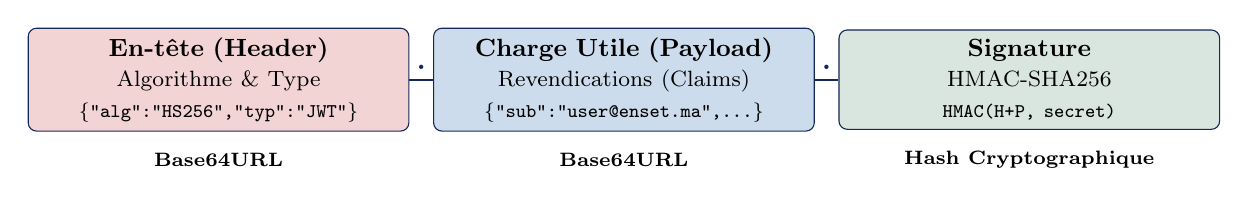
\begin{tikzpicture}[
    part/.style={rectangle, draw=darkblue, text width=4.6cm, text centered, minimum height=1.2cm, rounded corners=3pt, font=\small},
    labelstyle/.style={font=\scriptsize\bfseries}
]
\node[part, fill=javared!20] (header) {\textbf{En-tête (Header)}\\{\footnotesize Algorithme \& Type}\\{\scriptsize\texttt{\{"alg":"HS256","typ":"JWT"\}}}};
\node[part, fill=javablue!20, right=0.3cm of header] (payload) {\textbf{Charge Utile (Payload)}\\{\footnotesize Revendications (Claims)}\\{\scriptsize\texttt{\{"sub":"user@enset.ma",...\}}}};
\node[part, fill=javagreen!20, right=0.3cm of payload] (sig) {\textbf{Signature}\\{\footnotesize HMAC-SHA256}\\{\scriptsize\texttt{HMAC(H+P, secret)}}};

\draw[thick, darkblue] (header.east) -- node[above, font=\bfseries] {.} (payload.west);
\draw[thick, darkblue] (payload.east) -- node[above, font=\bfseries] {.} (sig.west);

\node[labelstyle, below=0.15cm of header] {Base64URL};
\node[labelstyle, below=0.15cm of payload] {Base64URL};
\node[labelstyle, below=0.15cm of sig] {Hash Cryptographique};

\end{tikzpicture}
\caption{Anatomie détaillée d'un jeton JSON Web Token (JWT)}
\label{fig:jwt-structure}
\end{figure}

\subsection{Implémentation du Service \texttt{JwtService}}
La classe \texttt{JwtService} regroupe la génération, l'extraction et la validation cryptographique des jetons avec l'API moderne de JJWT (0.13.0) :

\begin{lstlisting}[style=java, caption={Service de gestion des tokens (src/.../service/JwtService.java)}]
package org.example.tpjwtspring.service;

import io.jsonwebtoken.Claims;
import io.jsonwebtoken.Jwts;
import io.jsonwebtoken.io.Decoders;
import io.jsonwebtoken.security.Keys;
import org.springframework.beans.factory.annotation.Value;
import org.springframework.security.core.userdetails.UserDetails;
import org.springframework.stereotype.Service;
import javax.crypto.SecretKey;
import java.util.Date;

@Service
public class JwtService {

    @Value("${jwt.secret}")
    private String secret;

    @Value("${jwt.expiration}")
    private long expiration;

    private SecretKey getSigningKey() {
        byte[] keyBytes = Decoders.BASE64.decode(secret);
        return Keys.hmacShaKeyFor(keyBytes);
    }

    public String generateToken(UserDetails userDetails) {
        return Jwts.builder()
                .subject(userDetails.getUsername())
                .issuedAt(new Date())
                .expiration(new Date(System.currentTimeMillis() + expiration))
                .signWith(getSigningKey())
                .compact();
    }

    public String extractUsername(String token) {
        return extractAllClaims(token).getSubject();
    }

    private Claims extractAllClaims(String token) {
        return Jwts.parser()
                .verifyWith(getSigningKey())
                .build()
                .parseSignedClaims(token)
                .getPayload();
    }

    public boolean isTokenValid(String token, UserDetails userDetails) {
        final String username = extractUsername(token);
        return username.equals(userDetails.getUsername()) && !isTokenExpired(token);
    }

    private boolean isTokenExpired(String token) {
        return extractAllClaims(token).getExpiration().before(new Date());
    }
}
\end{lstlisting}

\subsection{Synthèse des Méthodes Cryptographiques}

\begin{table}[H]
\centering
\rowcolors{2}{rowgray}{white}
\begin{tabular}{|p{4.8cm}|p{3.2cm}|p{6cm}|}
\hline
\rowcolor{header}
\textcolor{white}{Méthode} &
\textcolor{white}{Retour} &
\textcolor{white}{Rôle et Opération} \\
\hline
\texttt{getSigningKey()} & \texttt{SecretKey} & Décode la clé Base64 et instancie la clé HMAC-SHA-256. \\
\texttt{generateToken(UserDetails)} & \texttt{String} & Injecte \texttt{sub}, \texttt{iat}, \texttt{exp} et signe le jeton. \\
\texttt{extractUsername(String)} & \texttt{String} & Récupère l'identifiant utilisateur (claim \texttt{sub}). \\
\texttt{extractAllClaims(String)} & \texttt{Claims} & Valide la signature HMAC et extrait le corps JSON. \\
\texttt{isTokenValid(token, user)} & \texttt{boolean} & Contrôle l'identité et la validité temporelle. \\
\texttt{isTokenExpired(String)} & \texttt{boolean} & Vérifie si l'instant actuel dépasse le timestamp \texttt{exp}. \\
\hline
\end{tabular}
\caption{Matrice fonctionnelle des méthodes de \texttt{JwtService}}
\label{tab:jwt-methods}
\end{table}



%------------------ Section 4 ------------------
\section{Gestion des Utilisateurs \& Spring Security}

\subsection{Intégration du Contrat Spring Security}
Pour charger les données d'identification lors de la vérification, la classe \texttt{CustomUserDetailsService} implémente l'interface de base \texttt{UserDetailsService} :

\begin{lstlisting}[style=java, caption={Service de chargement des identités (CustomUserDetailsService.java)}]
package org.example.tpjwtspring.service;

import org.example.tpjwtspring.entity.AppUser;
import org.example.tpjwtspring.repo.UserRepository;
import org.springframework.security.core.userdetails.User;
import org.springframework.security.core.userdetails.UserDetails;
import org.springframework.security.core.userdetails.UserDetailsService;
import org.springframework.security.core.userdetails.UsernameNotFoundException;
import org.springframework.stereotype.Service;

@Service
public class CustomUserDetailsService implements UserDetailsService {

    private final UserRepository userRepository;

    public CustomUserDetailsService(UserRepository userRepository) {
        this.userRepository = userRepository;
    }

    @Override
    public UserDetails loadUserByUsername(String username) 
            throws UsernameNotFoundException {

        AppUser user = userRepository
                .findByEmail(username)
                .orElseThrow(() ->
                    new UsernameNotFoundException("Utilisateur non trouve : " + username)
                );

        return User.builder()
                .username(user.getEmail())
                .password(user.getPassword())
                .roles(user.getRole())
                .build();
    }
}
\end{lstlisting}



%------------------ Section 5 ------------------
\section{Chaîne de Filtres et Pipeline d'Authentification}

\subsection{Diagrammes de Séquence des Flux Sécurisés}

\begin{figure}[H]
\centering
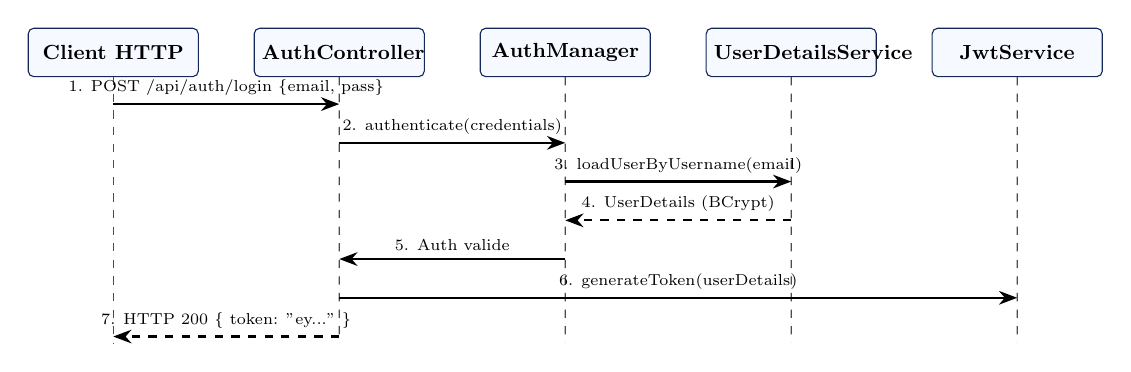
\begin{tikzpicture}[
    scale=0.82, every node/.style={transform shape},
    box/.style={rectangle, draw=darkblue, fill=lightblue!30, text centered, rounded corners=2pt, font=\small\bfseries, minimum height=0.75cm, text width=2.4cm},
    line/.style={draw=black!70, dashed}
]

% Participants Login
\node[box] (cl) at (0,0) {Client HTTP};
\node[box] (ctrl) at (3.5,0) {AuthController};
\node[box] (authMgr) at (7,0) {AuthManager};
\node[box] (uds) at (10.5,0) {UserDetailsService};
\node[box] (jwt) at (14,0) {JwtService};

\draw[line] (cl) -- ++(0,-4.5);
\draw[line] (ctrl) -- ++(0,-4.5);
\draw[line] (authMgr) -- ++(0,-4.5);
\draw[line] (uds) -- ++(0,-4.5);
\draw[line] (jwt) -- ++(0,-4.5);

\draw[-Stealth, thick] (0,-0.8) -- node[above, font=\scriptsize] {1. POST /api/auth/login \{email, pass\}} (3.5,-0.8);
\draw[-Stealth, thick] (3.5,-1.4) -- node[above, font=\scriptsize] {2. authenticate(credentials)} (7,-1.4);
\draw[-Stealth, thick] (7,-2.0) -- node[above, font=\scriptsize] {3. loadUserByUsername(email)} (10.5,-2.0);
\draw[-Stealth, thick, dashed] (10.5,-2.6) -- node[above, font=\scriptsize] {4. UserDetails (BCrypt)} (7,-2.6);
\draw[-Stealth, thick] (7,-3.2) -- node[above, font=\scriptsize] {5. Auth valide} (3.5,-3.2);
\draw[-Stealth, thick] (3.5,-3.8) -- node[above, font=\scriptsize] {6. generateToken(userDetails)} (14,-3.8);
\draw[-Stealth, thick, dashed] (3.5,-4.4) -- node[above, font=\scriptsize] {7. HTTP 200 \{ token: "ey..." \}} (0,-4.4);

\end{tikzpicture}
\caption{Cinématique d'authentification et émission du jeton}
\label{fig:seq-login}
\end{figure}

\begin{figure}[H]
\centering
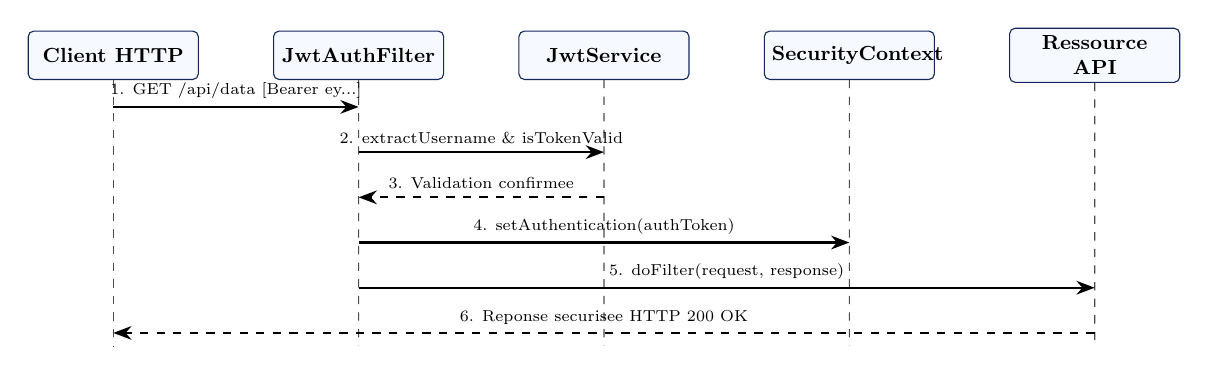
\begin{tikzpicture}[
    scale=0.82, every node/.style={transform shape},
    box/.style={rectangle, draw=darkblue, fill=lightblue!30, text centered, rounded corners=2pt, font=\small\bfseries, minimum height=0.75cm, text width=2.4cm},
    line/.style={draw=black!70, dashed}
]

% Participants Requête protégée
\node[box] (cl) at (0,0) {Client HTTP};
\node[box] (flt) at (3.8,0) {JwtAuthFilter};
\node[box] (jwt) at (7.6,0) {JwtService};
\node[box] (ctx) at (11.4,0) {SecurityContext};
\node[box] (ep) at (15.2,0) {Ressource API};

\draw[line] (cl) -- ++(0,-4.5);
\draw[line] (flt) -- ++(0,-4.5);
\draw[line] (jwt) -- ++(0,-4.5);
\draw[line] (ctx) -- ++(0,-4.5);
\draw[line] (ep) -- ++(0,-4.5);

\draw[-Stealth, thick] (0,-0.8) -- node[above, font=\scriptsize] {1. GET /api/data [Bearer ey...]} (3.8,-0.8);
\draw[-Stealth, thick] (3.8,-1.5) -- node[above, font=\scriptsize] {2. extractUsername \& isTokenValid} (7.6,-1.5);
\draw[-Stealth, thick, dashed] (7.6,-2.2) -- node[above, font=\scriptsize] {3. Validation confirmee} (3.8,-2.2);
\draw[-Stealth, thick] (3.8,-2.9) -- node[above, font=\scriptsize] {4. setAuthentication(authToken)} (11.4,-2.9);
\draw[-Stealth, thick] (3.8,-3.6) -- node[above, font=\scriptsize] {5. doFilter(request, response)} (15.2,-3.6);
\draw[-Stealth, thick, dashed] (15.2,-4.3) -- node[above, font=\scriptsize] {6. Reponse securisee HTTP 200 OK} (0,-4.3);

\end{tikzpicture}
\caption{Cinématique d'interception et validation du jeton par le filtre}
\label{fig:seq-validation}
\end{figure}

\subsection{Configuration de Sécurité (\texttt{SecurityFilterChain})}
Dans Spring Security 6, la configuration est déclarée via un bean \texttt{SecurityFilterChain} :

\begin{lstlisting}[style=java, caption={Configuration de sécurité stateless (SecurityConfig)}]
@Configuration
@EnableWebSecurity
public class SecurityConfig {

    private final JwtAuthenticationFilter jwtAuthFilter;
    private final CustomUserDetailsService userDetailsService;

    public SecurityConfig(JwtAuthenticationFilter jwtAuthFilter, 
                          CustomUserDetailsService userDetailsService) {
        this.jwtAuthFilter = jwtAuthFilter;
        this.userDetailsService = userDetailsService;
    }

    @Bean
    public SecurityFilterChain securityFilterChain(HttpSecurity http) throws Exception {
        return http
            .csrf(csrf -> csrf.disable()) // Desactive car pas de session ni cookies
            .sessionManagement(sm -> sm.sessionCreationPolicy(SessionCreationPolicy.STATELESS))
            .authorizeHttpRequests(auth -> auth
                .requestMatchers("/api/auth/**", "/h2-console/**").permitAll()
                .anyRequest().authenticated()
            )
            .headers(h -> h.frameOptions(fo -> fo.disable())) // Console H2
            .addFilterBefore(jwtAuthFilter, UsernamePasswordAuthenticationFilter.class)
            .build();
    }

    @Bean
    public PasswordEncoder passwordEncoder() {
        return new BCryptPasswordEncoder();
    }
}
\end{lstlisting}



%------------------ Section 6 ------------------
\section{Spécification des Endpoints, Tests et Validation}

\subsection*{Exemples de commandes utilisées}

\definecolor{header}{RGB}{40,60,120}
\definecolor{rowgray}{RGB}{245,245,245}
\definecolor{lightblue}{RGB}{225,235,255}

\begin{table}[H]
\centering
\rowcolors{2}{rowgray}{white}
\begin{tabular}{|p{4.8cm}|p{9.2cm}|}
\hline
\rowcolor{header}
\textcolor{white}{Commande} &
\textcolor{white}{Description} \\
\hline

\rowcolor{lightblue}
\multicolumn{2}{|l|}{\textbf{Commandes de Build Maven}} \\
\hline
\texttt{./mvnw test-compile} & Compile les sources et vérifie les dépendances. \\
\texttt{./mvnw spring-boot:run} & Lance l'application sur le port local \texttt{8080}. \\
\texttt{./mvnw clean package} & Construit l'archive exécutable JAR. \\
\hline

\rowcolor{lightblue}
\multicolumn{2}{|l|}{\textbf{Commandes d'Appel HTTP (cURL)}} \\
\hline
\texttt{curl -X POST /api/auth/register} & Inscription d'un nouvel utilisateur avec JSON \texttt{\{email, pass\}}. \\
\texttt{curl -X POST /api/auth/login} & Connexion et récupération du jeton JWT. \\
\texttt{curl -H "Authorization: Bearer <T>"} & Requête authentifiée vers une ressource sécurisée. \\
\hline

\end{tabular}
\caption{Commandes utilisées durant le TP}
\label{tab:commandes}
\end{table}

\subsection{Matrice des Endpoints de l'API}

\begin{table}[H]
\centering
\rowcolors{2}{rowgray}{white}
\begin{tabular}{|l|l|p{3.8cm}|p{2.6cm}|c|}
\hline
\rowcolor{header}
\textcolor{white}{Méthode} &
\textcolor{white}{URI Endpoint} &
\textcolor{white}{En-tête Requise} &
\textcolor{white}{Payload Requis} &
\textcolor{white}{Statut} \\
\hline
\texttt{POST} & \texttt{/api/auth/register} & \texttt{Content-Type: app/json} & \texttt{\{email, pass\}} & 200 / 201 \\
\texttt{POST} & \texttt{/api/auth/login} & \texttt{Content-Type: app/json} & \texttt{\{email, pass\}} & 200 OK \\
\texttt{GET} & \texttt{/api/user/profile} & \texttt{Authorization: Bearer <T>} & Aucun & 200 OK \\
\texttt{GET} & \texttt{/h2-console} & Authentification web & Identifiants H2 & 200 OK \\
\hline
\end{tabular}
\caption{Spécification des endpoints REST de l'API d'authentification}
\label{tab:endpoints}
\end{table}

\subsection{Validation de la Compilation et Requête Postman}

\begin{lstlisting}[style=console, caption={Compilation sans erreur du projet avec Maven Wrapper}]
$ ./mvnw test-compile
[INFO] Scanning for projects...
[INFO] ---------------------< org.example:tp-jwt-spring >----------------------
[INFO] Building tp-jwt-spring 0.0.1-SNAPSHOT
[INFO] Compiling 8 source files with javac [debug parameters release 21]
[INFO] Compiling 1 source file with javac to target/test-classes
[INFO] ------------------------------------------------------------------------
[INFO] BUILD SUCCESS
[INFO] Total time:  10.963 s
[INFO] ------------------------------------------------------------------------
\end{lstlisting}

\begin{figure}[H]
\centering
\begin{tcolorbox}[colback=black!85, colframe=black, arc=3mm, width=0.92\linewidth]
\color{green!80!white}\ttfamily\small
POST /api/auth/login HTTP/1.1\\
Host: localhost:8080\\
Content-Type: application/json\\[0.3cm]
\{\\
\ \ "email": "ayoub.elhouani@enset-media.ac.ma",\\
\ \ "pass": "SecretP@ssw0rd2026"\\
\}\\[0.4cm]
\color{yellow!90!white}HTTP/1.1 200 OK\\
Content-Type: application/json\\[0.3cm]
\color{cyan!80!white}\{\\
\ \ "token": "eyJhbGciOiJIUzI1NiJ9.eyJzdWIiOiJheW91Yi5lbGhvdWFuaU...\\
\ \ \ \ \ \ \ \ \ \ ...NzYwNDc2MDAwLCJleHAiOjE3NjA0Nzk2MDB9.7q0\_Z\_w9mK18a..."\\
\}
\end{tcolorbox}
\caption{Exemple de requête d'authentification et obtention du jeton Bearer}
\label{fig:postman-capture}
\end{figure}

%------------------ Section 7 ------------------
\section{Sécurité Avancée, Révocation \& Scalabilité}

\subsection{Refresh Tokens \& Révocation avec Cache Redis}
L'inconvénient fondamental d'un token JWT sans état est l'impossibilité de l'invalider avant son terme s'il est dérobé. La solution industrielle consiste à employer un \textbf{Access Token} à durée courte (15 minutes) couplé à un \textbf{Refresh Token} à durée longue (7 jours) stocké dans un cookie \texttt{HttpOnly} et révocable via une liste noire en cache mémoire \textbf{Redis} :

\begin{figure}[H]
\centering
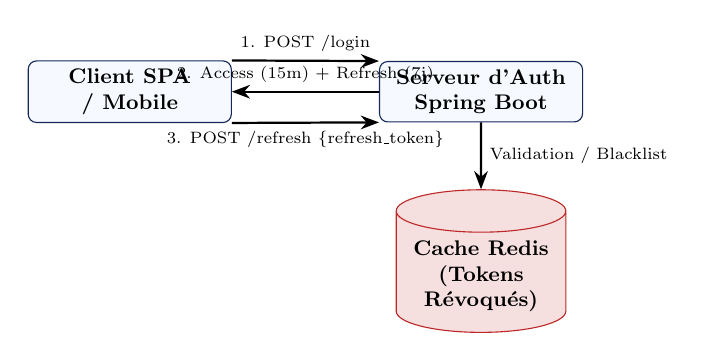
\begin{tikzpicture}[
    scale=0.85, every node/.style={transform shape},
    rect/.style={rectangle, draw=darkblue, fill=lightblue!30, text centered, rounded corners=3pt, font=\small\bfseries, minimum height=0.9cm, text width=2.8cm},
    store/.style={cylinder, draw=javared, fill=javared!15, shape border rotate=90, aspect=0.25, text centered, font=\small\bfseries, minimum height=1.1cm, text width=2.3cm}
]

\node[rect] (client) {Client SPA / Mobile};
\node[rect, right=2.2cm of client] (auth) {Serveur d'Auth\\Spring Boot};
\node[store, below=1cm of auth] (redis) {Cache Redis\\(Tokens Révoqués)};

\draw[-Stealth, thick] (client.north east) -- node[above, font=\scriptsize] {1. POST /login} (auth.north west);
\draw[-Stealth, thick] (auth.west) -- node[above, font=\scriptsize] {2. Access (15m) + Refresh (7j)} (client.east);
\draw[-Stealth, thick] (client.south east) -- node[below, font=\scriptsize] {3. POST /refresh \{refresh\_token\}} (auth.south west);
\draw[-Stealth, thick] (auth) -- node[right, font=\scriptsize] {Validation / Blacklist} (redis);

\end{tikzpicture}
\caption{Architecture avec Refresh Token et Blacklisting via Redis}
\label{fig:refresh-token}
\end{figure}

\subsection{Signature Symétrique (HMAC) vs Asymétrique (RSA)}
Pour des microservices d'envergure, l'algorithme asymétrique \textbf{RS256} (RSA avec SHA-256) permet au serveur d'authentification de détenir la \textbf{clé privée} pour émettre les jetons, tandis que les microservices tiers vérifient la signature avec la seule \textbf{clé publique}, sans risque de compromission de la clé maîtresse.



%------------------ Conclusion ------------------
\section*{Conclusion}
\addcontentsline{toc}{section}{Conclusion}
Ce travail pratique a permis de consolider la mise en place d'une architecture d'authentification moderne et sans état (\textit{Stateless}) sous Spring Boot et Spring Security 6 avec la bibliothèque JJWT.

Le découplage des responsabilités entre le modèle JPA \texttt{AppUser}, la couche d'accès aux données \texttt{UserRepository}, le chargement des identités (\texttt{CustomUserDetailsService}) et la signature des jetons (\texttt{JwtService}) garantit une modularité rigoureuse, une haute sécurité et une scalabilité optimale.

\end{document}
